\documentclass[]{book}

%These tell TeX which packages to use.
\usepackage{array,epsfig}
\usepackage{amsmath}
\usepackage{amsfonts}
\usepackage{amssymb}
\usepackage{amsxtra}
\usepackage{amsthm}
\usepackage{mathrsfs}
\usepackage{color}

%Here I define some theorem styles and shortcut commands for symbols I use often
\theoremstyle{definition}
\newtheorem{defn}{Definition}
\newtheorem{thm}{Theorem}
\newtheorem{cor}{Corollary}
\newtheorem*{rmk}{Remark}
\newtheorem{lem}{Lemma}
\newtheorem*{joke}{Joke}
\newtheorem{ex}{Example}
\newtheorem*{soln}{Solution}
\newtheorem{prop}{Proposition}

\newcommand{\lra}{\longrightarrow}
\newcommand{\ra}{\rightarrow}
\newcommand{\surj}{\twoheadrightarrow}
\newcommand{\graph}{\mathrm{graph}}
\newcommand{\bb}[1]{\mathbb{#1}}
\newcommand{\Z}{\bb{Z}}
\newcommand{\Q}{\bb{Q}}
\newcommand{\R}{\bb{R}}
\newcommand{\C}{\bb{C}}
\newcommand{\N}{\bb{N}}
\newcommand{\M}{\mathbf{M}}
\newcommand{\m}{\mathbf{m}}
\newcommand{\MM}{\mathscr{M}}
\newcommand{\HH}{\mathscr{H}}
\newcommand{\Om}{\Omega}
\newcommand{\Ho}{\in\HH(\Om)}
\newcommand{\bd}{\partial}
\newcommand{\del}{\partial}
\newcommand{\bardel}{\overline\partial}
\newcommand{\textdf}[1]{\textbf{\textsf{#1}}\index{#1}}
\newcommand{\img}{\mathrm{img}}
\newcommand{\ip}[2]{\left\langle{#1},{#2}\right\rangle}
\newcommand{\inter}[1]{\mathrm{int}{#1}}
\newcommand{\exter}[1]{\mathrm{ext}{#1}}
\newcommand{\cl}[1]{\mathrm{cl}{#1}}
\newcommand{\ds}{\displaystyle}
\newcommand{\vol}{\mathrm{vol}}
\newcommand{\cnt}{\mathrm{ct}}
\newcommand{\osc}{\mathrm{osc}}
\newcommand{\LL}{\mathbf{L}}
\newcommand{\UU}{\mathbf{U}}
\newcommand{\support}{\mathrm{support}}
\newcommand{\AND}{\;\wedge\;}
\newcommand{\OR}{\;\vee\;}
\newcommand{\Oset}{\varnothing}
\newcommand{\st}{\ni}
\newcommand{\wh}{\widehat}

%Pagination stuff.
\setlength{\topmargin}{-.3 in}
\setlength{\oddsidemargin}{0in}
\setlength{\evensidemargin}{0in}
\setlength{\textheight}{9.in}
\setlength{\textwidth}{6.5in}
\pagestyle{empty}



\begin{document}


\subsection*{Exo 3.1.1}
\subsubsection*{Q1}
(a) $$\overrightarrow{u} = 
\left\{ 
\begin{array}{l}
u_x = \Vert \overrightarrow{u} \Vert cos(\alpha) \\
u_y = \Vert \overrightarrow{u} \Vert sin(\alpha) \\
\end{array}
\right. 
$$

(b)
$$\overrightarrow{w} = 
\left\{ 
\begin{array}{l}
w_x = \Vert \overrightarrow{w} \Vert sin(\beta) \\
w_y = \Vert \overrightarrow{w} \Vert cos(\beta) \\
\end{array}
\right. 
$$

\subsubsection*{Q2}
\begin{figure}[h!]
  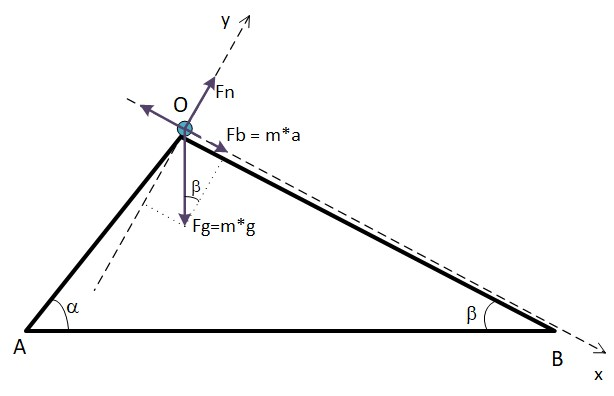
\includegraphics[width=0.8\linewidth]{exo3_1_1_pente.jpg}
  \caption{Pente}
\end{figure}

On va travailler dans le rep\`ere orthonorm\'ee $Oxy$ parall\`ele au plan inclin\'e.

Il y a 3 forces appliqu\'ees sur l'objet :
\begin{itemize}
\item la force gravitationnelle $\overrightarrow{F_g} = m\overrightarrow{g}$
\item la force normale au plan $\overrightarrow{F_n}$ 
\item la force r\'esultante $\overrightarrow{F_b} = m\overrightarrow{a_b}$
\end{itemize}

Dans le rep\`ere orthonorm\'ee $Oxy$, les 3 forces ont les valeurs suivantes:
$$\overrightarrow{w} = 
\left\{ 
\begin{array}{l l l }
\overrightarrow{F_n} & \overrightarrow{F_b} & \overrightarrow{F_g} \\ 
 (0, \Vert \overrightarrow{F_n} \Vert) & (-m * \overrightarrow{a_b},0) & (m*\overrightarrow{g}*sin(\beta), -m*\overrightarrow{g}*cos(\beta)) \\
\end{array}
\right. 
$$

La somme des forces est nulle(2nd loi de Newton).
$$ \sum{\overrightarrow{F}} = 0$$
$$ \overrightarrow{F_g} + \overrightarrow{F_n} + \overrightarrow{F_b} = 0$$

$$\sum{\overrightarrow{F}} = 
\left\{ 
\begin{array}{l}
\sum{\overrightarrow{F_x}} =  0 +  -m * \overrightarrow{a_b},0) + m*\overrightarrow{g}*sin(\beta) \\
\sum{\overrightarrow{F_y}} = \Vert \overrightarrow{F_n} \Vert) + 0 + -m*\overrightarrow{g}*cos(\beta)) \\
\end{array}
\right. 
= 0
$$

$$
\left\{ 
\begin{array}{l}
m * \overrightarrow{a_b},0) = m*\overrightarrow{g}*sin(\beta) \\
\Vert \overrightarrow{F_n} \Vert) = m*\overrightarrow{g}*cos(\beta)) \\
\end{array}
\right. 
$$

Donc l'acc\'el\'eration de la boule B est $g*sin(\beta))$.
De m\^eme pour l'acc\'el\'eration de la boule A est $g*sin(\alpha))$.

\subsubsection*{Q3}
Soit $h$ la hauteur du triangle. La longueur $OA = \frac{h}{sin(\alpha)}$ et $OB = \frac{h}{sin(\beta)}$. Comme l'acc\'el\'eration est constante 
la distance parcourue apr\`es $t$ secondes est $d = \frac{1}{2}.a.t^2$ avec $a = g*sin(\alpha)$ et $d = OA$ pour la boule A . Donc
$$ t = \sqrt{\frac{2.d}{a}}$$.
$$ t = \sqrt{\frac{2.OA}{g.sin(\alpha)}}$$.
$$ t = \sqrt{\frac{2.\frac{h}{sin(\alpha)}}{g.sin(\alpha)}}$$.
$$ t = \sqrt{\frac{2.h}{g.sin^2(\alpha)}}$$.

De m\^eme, le temps de parcours pour la boule B; $ t = \sqrt{\frac{2.h}{g.sin^2(\beta)}}$.
  

\subsubsection*{Q4}
L'acc\'el\'eration est constante donc la vitesse \`a l'instant $t$ est $v(t) = a.t$ avec $a = g.sin(\alpha)$ et $ t = \sqrt{\frac{2.h}{g.sin^2(\alpha)}}$.
Donc la vitesse de la boule A est $g.sin(\alpha) . \sqrt{\frac{2.h}{g.sin^2(\alpha)}} = \sqrt{2.h.g}$ et la boule B a la m\^eme vitesse $\sqrt{2.h.g}$

\end{document}

